\documentclass[table,usenames,dvipsnames]{beamer}

\usepackage[english]{babel}
\usepackage[utf8]{inputenc}
\usepackage{listings}
\usepackage{datetime}
\usepackage{graphics}
\usepackage{fancybox}
\usepackage{color}
\usepackage[normalem]{ulem}
\usepackage{tikz}
\usepackage{listings}
\usetikzlibrary{shapes,arrows}
\usetheme{CambridgeUS}
\usecolortheme{seagull}

\DefineNamedColor{named}{Purple}{cmyk}{0.52,0.97,0,0.55}
\setbeamertemplate{itemize item}[triangle]
\setbeamercolor{title}{fg=Purple}
\setbeamercolor{frametitle}{fg=Purple}
\setbeamercolor{itemize item}{fg=Purple}
\setbeamercolor{section number projected}{bg=Purple,fg=white}
\setbeamercolor{subsection number projected}{bg=Purple}

\renewcommand{\dateseparator}{.}
\newcommand{\todayiso}{\twodigit\day \dateseparator \twodigit\month \dateseparator \the\year}
\newcommand{\shell}[1]{\texttt{#1}}
\definecolor{LightGray}{gray}{0.9}

\title{Osnove korištenja operacijskog sustava Linux}
\subtitle{07. Procesi i ljuske}
\author[Dominik Barbarić]{Dominik Barbarić\\ \small{Nositelj: dr. sc. Stjepan Groš}}
\institute[FER]{Sveučilište u Zagrebu \\
				Fakultet elektrotehnike i računarstva}
				
\date{\todayiso}

\begin{document}
{
\setbeamertemplate{headline}[] % still there but empty
\setbeamertemplate{footline}{}

\begin{frame}
\maketitle
\end{frame}
}

\begin{frame}
\frametitle{Sadržaj}
\tableofcontents
\end{frame}

\section{Procesi}
\begin{frame}[t]
\frametitle{Proces i program}
\begin{itemize}
  \item Program
  \begin{itemize}
    \item Datoteka s izvršnim kodom
    \item Primjer: \shell{/bin/bash} je program
  \end{itemize}
  \item Proces
  \begin{itemize}
    \item Pokretanjem programa na računalu nastaje \emph{proces}
    \item Za proces su vezani izvršni kod programa te svi podaci vezani uz izvršavanje programa (podaci u memoriji i u ostalim resursima)
    \item Svaki proces posjeduje jedinstveni identifikator - PID (\emph{process identifier})
  \end{itemize}
\end{itemize}
\end{frame}

\subsection{Ispis procesa}
\begin{frame}[t]
\frametitle{Ispis procesa}
\begin{itemize}
 
  \item Ispis procesa obavlja se s naredbom \shell{ps} 
  \begin{itemize}
  	\item \emph{process status}
  	\item ako se pokrene bez argumenata i opcija ispisuju se procesi vezani za trenutni terminal
  \end{itemize}
  \item \shell{ps} prihvaća tri vrste opcija: Unix, BSD, GNU opcije
  \item[]
	\item Zadatak
	\begin{itemize}
	  	\item U man stranicama proučiti opcije \shell{ps} naredbe.
  	\end{itemize}
\end{itemize}
\end{frame}

\begin{frame}[t]
	\frametitle{Ispis procesa}
	\begin{itemize}
		\item Ispis naredbe \shell{ps} sadrži:
		\begin{tabular}{l l}
			PID   & Process ID \\
			TTY   & TTY (terminal) za koji je proces vezan \\
			TIME  & Ukupno vrijeme izvršavanja  \\
			CMD   & Naredba kojom je proces pokrenut (put do programa, \\ & bez argumenata)
		\end{tabular}
		\item[]
		\item Dodatne informacije o procesima korištenjem opcije \shell{-f}
		\begin{tabular}{l l}
			UID   & Vlasnik procesa \\
			PPID  &   Roditelj procesa \\
			CMD   &   Naredba s argumentima
		\end{tabular}
	\end{itemize}
\end{frame}

\begin{frame}[t]
	\frametitle{Ispis procesa}
	\begin{itemize}
		\item Korisne opcije \shell{ps} naredbe
		\begin{tabular}{l l}
			\shell{-e}        & ispis svih procesa u sustavu \\
			\shell{-f}        & dodatne informacije o procesima \\
			\shell{-o}        & zadavanje formata ispisa \\
			\shell{-{}-sort}  & sortiranje ispisa (po PID ako nije drugačije navedeno)
		\end{tabular} 
		\item[]
		\item[] Primjer: Ispis procesa s prikazom navedenih atributa i sortiranjem
		\item[] \hspace{40pt} \shell{ps -eo pid,ppid,user,args,nice --sort user}
	\end{itemize}
\end{frame}

\begin{frame}[t]
	\frametitle{Ispis procesa}
	\begin{itemize}
		\item S argumentom \shell{u} dobivamo pregled resursa koje procesi zauzimaju
		\item[]
		\begin{tabular}{l l}
			\%CPU   & Zauzeće procesora  \\
			\%MEM   & Zauzeće radne memorije \\ 
			VSZ     & Veličina virtualne memorije \\
			STAT    & Trenutno stanje procesa \\
			START   & Vrijeme pokretanja procesa
		\end{tabular}
	\end{itemize}
\end{frame}

\begin{frame}[t]
	\frametitle{Stanja procesa}
	\begin{itemize}
		\item Procesi mogu poprimiti sljedeća stanja:
		\begin{tabular}{l l}
			\\
			\textbf{R}  & \emph{running} - aktivni proces \\
			\textbf{S}  & \emph{sleeping} - neaktivan 20 sekundi ili manje \\
			\textbf{I}  & \emph{idle} - neaktivan više od 20 sekundi \\
			\textbf{T}  & \emph{stopped} - zaustavljen proces \\
			\textbf{Z}  & \emph{zombie} - proces koji je završio, ali je još uvijek upisan \\ & u tablicu procesa
		\end{tabular}
	\end{itemize}
\end{frame}

\section{Signali}
\begin{frame}[t]
	\frametitle{Signali}
	\begin{itemize}
		\item \emph{Signal} je metoda komunikacije između procesa (IPC - Inter-process communication)
		\item Pojava signala izaziva prekid u radu procesa
		\item Ovisno o vrsti primljenog signala proces ili jezgra operativnog sustava obrađuju prekid
		\begin{itemize}
			\item Proces može za primljeni signal obraditi funkciju koja se definira kao \emph{signal handler}. Ako nije definirana signal handler funkcija izvršava se zadana radnja (ovisno o vrsti signala)			\item Po završetku obrade proces nastavlja s normalnim izvršavanjem (osim ako u prekidu nije okončan)
		\end{itemize}
	\end{itemize}
\end{frame}


\defverbatim[colored]\makeset{
\begin{lstlisting}[language=C, basicstyle=\tiny\ttfamily, showstringspaces=false, keywordstyle=\color{blue}]
#include <stdio.h>
#include <stdlib.h>
#include <signal.h>

void signal_handle(int sig_code){
	if (sig_code == SIGINT){
		printf("Primljen INT. Kraj programa!\n");
		exit(0);
	}
	else if (sig_code == SIGUSR1)
		printf("Primiljen USR1\n");
}

int main(){
	if (signal(SIGINT, signal_handle) == SIG_ERR)
		exit(1);
	if (signal(SIGUSR1, signal_handle) == SIG_ERR)
		exit(1);
		
	while(1)
		sleep(1);
		
	return 0;
}
\end{lstlisting}
}

\begin{frame}[t]
	\frametitle{Signal handler primjer}
	\begin{block}{main.c}
		\makeset
	\end{block}
\end{frame}

\begin{frame}[t]
	\frametitle{Signali}
	\begin{itemize}
		\item U UNIX sustavima svaka vrsta signala uz naziv ima i brojčanu oznaku
	\end{itemize}
	\begin{table}[h]
		\rowcolors{1}{White}{LightGray}
		\begin{tabular}{l l l}
			\rowcolor{BlueViolet!20}Naziv signala & Kod & Značenje \\
			SIGHUP & 1 & \emph{Hangup} - Ugašen terminal u kojem se \\ & & proces odvijao \\
			SIGINT & 2 & \emph{Terminal interrupt} - Signal s terminala. \\ & & Aktivira se s CTRL+C \\
			SIGTERM & 15 & \emph{Terminate} - Programsko gašenje procesa \\
			SIGKILL & 9 & \emph{Kill} - Trenutačno gašenje procesa \\
			SIGUSR1 & 10 & \emph{User defined 1} 
		\end{tabular}
	\end{table}
	\begin{itemize}
		\item Popis svih signala: \shell{man 7 signal}
		\item Signali su se kroz razne standardizacije mijenjali. Uočite u \shell{man} stranicama da je \shell{SIGUSR1} u ranijim sustavima imao 3 koda
	\end{itemize}
\end{frame}

\subsection{Slanje signala}
\begin{frame}[t]
	\frametitle{Slanje signala}
	\begin{itemize}
		\item Signali se u komandnoj liniji šalju naredbom \shell{kill}
		\begin{itemize}
			\item[] \shell{kill [-<kod signala>] <PID>}
			\item[]
			\item Ako kod signala nije naveden kao argument \shell{kill} će poslati signal SIGTERM
		\end{itemize}
		
		\item[]
		\item Neke kombinacije tipki također mogu poslati signale (npr. CTRL+C)
	\end{itemize}
\end{frame}


\subsection{Child procesi}
\begin{frame}[t]
	\frametitle{Child procesi}
	\begin{itemize}
		\item Proces može pokrenuti drugi proces. Prvi proces je tada \emph{roditelj}, a svi procesi koje je pozvao su njegova \emph{djeca}.
		\item Child procesi sadrže dodatni podatak - PPID – \emph{parent PID} koji pokazuje na njihove roditelje
	  	\item[]
	  	\item Svi procesi u sustavu su djeca nekog drugog procesa
		  	\begin{itemize}
		  		\item Iznimka je \emph{init} proces s PID = 1 kojeg stvara kernel pokretanju OS-a
		  		\item Proces \emph{init} je roditelj svim ostalim procesima
		  	\end{itemize}
		\item Gašenje roditeljskog procesa gasi i sve njegove child procese.
	\end{itemize}
\end{frame}

\begin{frame}[t]
\frametitle{Child procesi}
\framesubtitle{Process management funkcije}
\begin{itemize}
  \item Pokretanje novog procesa ostvaruje se pozivanjem funkcije fork()
  \item fork() će stvoriti novi proces iz roditelja pozivajući \emph{isti} program
  \item[]
  \item Prilikom izvršavanja programa u novom procesu ponovno se nailazi na funkciju fork() koja vraća vrijednost:
  \begin{itemize}
    \item \emph{PID novog procesa}, ako je fork() pozvan iz roditeljskog procesa
    \item \emph{0}, ako je fork() pozvan iz child procesa
  \end{itemize}
\end{itemize}
\end{frame}

\defverbatim[colored]\makeset{
\begin{lstlisting}[language=C, basicstyle=\tiny\ttfamily, showstringspaces=false, keywordstyle=\color{blue}]
#include <unistd.h>
#include <stdio.h>

int main(){
	int pid = fork();
	
	if (pid == 0)
		printf("Ovo je child proces!\n");
	else if (pid != -1)
		printf("Ovo je roditelj. Pozvan je child proces s PID %d\n", pid);
	else {
		printf("Fork nije uspio.\n");
		return 1;
	}
	
	return 0;
}
\end{lstlisting}
}

\begin{frame}[t]
	\frametitle{fork() primjer}
	\begin{block}{main.c}
		\makeset
	\end{block}
	\begin{block}{Izlaz}{\small \ttfamily
		Ovo je roditelj. Pozvan je child proces s PID 4924.\\
		Ovo je child proces!
	}\end{block}
\end{frame}
 
\begin{frame}[t]
	\frametitle{Child procesi}
	\framesubtitle{Process management funkcije}
	\begin{itemize}
		\item Funkcija wait() čeka da child proces pozvan funkcijom fork() završi s izvođenjem.
		\begin{itemize}
			\item wait() će, ako nije drugačije zadano čekati završetak prvog pozvanog djeteta
			\item wait() u jeziku C može prihvatiti izlaznu vrijednost programa:
			\item[] \shell{int status; wait(\&status);}
		\end{itemize}
		\item[]
		\item Nakon završetka izvođenja child procesa, on će ostati u stanju \emph{zombie} dok ga roditeljski proces ne "uhvati" wait() pozivom
		\item waitpid() će čekati završetak procesa čiji PID zadajemo argumentom
		\item[]
		\item Zadatak:
		\begin{itemize}
			\item Proučiti sva man poglavlja za fork, wait i waitpid.
		\end{itemize}
	\end{itemize}
\end{frame}

\defverbatim[colored]\makeset{
\begin{lstlisting}[language=C, basicstyle=\tiny\ttfamily, showstringspaces=false, keywordstyle=\color{blue}]
...
	if (pid == 0)
		printf("Ovo je child proces!\n");
	else if (pid != -1){
		printf("Ovo je roditelj. Pozvan je child proces s PID %d\n", pid);
		wait();
		printf("Child proces je zavrsio s izvodjenjem\n");
	} else {
		printf("Fork nije uspio.\n");
		return 1;
	}
...
\end{lstlisting}
}

\begin{frame}[t]
	\frametitle{wait() primjer}
	Dogradimo prethodni primjer:
	\begin{block}{main.c}
		\makeset
	\end{block}
	\begin{block}{Izlaz}{\small \ttfamily
		Ovo je roditelj. Pozvan je child proces s PID 4924\\
		Ovo je child proces!\\
		Child proces je završio s izvođenjem
	}\end{block}
\end{frame}

\begin{frame}[t]
	\frametitle{Dodatne naredbe}
	\framesubtitle{Pretraga i ispis procesa}
	\begin{itemize}
		\item \shell{pgrep} pretražuje procese po imenu i drugim atributima
		\item \shell{pstree} ispisuje stablo svih procesa na sustavu
		\item Naredba \shell{top} prikazuje stanje svih procesa u real-time sučelju
		\begin{itemize}
			\item Naprednija verzija ovog sučelja - \shell{htop}
		\end{itemize}
		\item[]
	\end{itemize}
	
	Podrazumijevane vrijednosti naredbe \shell{top}
	\begin{itemize} 
		\item Osvježavanje se obavlja svake 3 sekunde
		\begin{itemize}
			\item Učestalost osvježavanja se mijenja tipkom \shell{i}
		\end{itemize}
		\item Procesi su poredani po zauzeću procesora
		\begin{itemize}
			\item Tipka \shell{M} - sortiranje po zauzeću memorije
			\item Tipka \shell{S} - sortiranje po zauzeću procesora
		\end{itemize}
	\end{itemize}
\end{frame}

\begin{frame}[t]
	\frametitle{Dodatne naredbe}
	\framesubtitle{Slanje signala}
	Za slanje signala procesima po nazivu procesa postoji nekoliko naredbi
	\begin{itemize}
		\item \shell{killall} - šalje signal procesima pod točno navedenim nazivom
		\begin{itemize}
			\item Signal se šalje svim procesima pod tim imenom
			\item Primjer: \shell{killall -SIGKILL dd} \\ šalje SIGKILL svim dd procesima
		\end{itemize}
		\item \shell{pkill} - šalje signal procesima pretragom naziva po zadanom uzorku
		\begin{itemize}
			\item Primjer: \shell{pkill -SIGKILL dd} \\ šalje SIGKILL svim procesima koji u nazivu sadrže dd (npr. proces \shell{ddclient} bi ovdje također bio prekinut)
		\end{itemize}
	\end{itemize}
\end{frame}


\begin{frame}[t]
\frametitle{Prioriteti}
\begin{itemize}
  \item Kod rezerviranja CPU vremena procesi imaju prioritet - \emph{niceness}
  \begin{itemize}
    \item -20 - najviši prioritet
    \item +19 - najniži prioritet
    \item[]
    \item Većina korisničkih programa ima isti niceness - 0
    \item Procesi \emph{realtime} prioriteta imaju prednost nad ostalima bez obzira na niceness
  \end{itemize}
  \item[]
  \item Naredbom \shell{nice} procesi se pokreću sa višim ili nižim prioritetom
  \begin{itemize}
    \item \shell{renice} mijenja prioritet postojećeg procesa ili grupe procesa
  \end{itemize}
\end{itemize}
\end{frame}


\section{Ljuska}
\begin{frame}[t]
	\frametitle{Ljuska}
	\begin{itemize}
		\item Ljuska je korisničko sučelje prema operacijskom sustavu
		\item Program koji se prvi pokreće paljenjem terminala
		\begin{itemize}
			\item Ljuska tada ima ulaz i izlaz vezan na terminal
		\end{itemize}
		\item Ljuska pokreće procese i usmjerava njihove ulaze i izlaze
		\item Ljuska može omogućiti automatizaciju (skripte)
	\end{itemize}
\end{frame}

\begin{frame}[t]
	\frametitle{Ljuska}
	\begin{itemize}
		\item Ljuske u Linuxu
		\begin{itemize}
			\item Popis ljuski dostupnih na sustavu - \shell{/etc/shells}
			\item sh, bash, csh, ksh, \ldots
		\end{itemize}
		\item[]
		\item Zadana ljuska za korisnika se zadaje u \shell{/etc/passwd}
		\item Neke (starije) distribucije podržavaju promjenu ljuske s \shell{chsh}
	\end{itemize}
\end{frame}


\begin{frame}[t]
	\frametitle{Ljuska}
	\framesubtitle{Bash}
	\begin{itemize}
		\item Najraširenija ljuska na Linux sustavima - \shell{bash}
		\begin{itemize}
			\item \emph{Bourne again shell}
		\end{itemize}
		\item Nadogradnja \shell{sh} ljuske (\emph{Bourne shell})
		\item[]
		\item Bash uvodi
		\begin{itemize}
			\item upravljanje poslovima (\shell{jobs}, \shell{bg}, \shell{fg})
			\item neograničenu povijest naredbi
			\item pseudonime (\emph{alias})
		\end{itemize}
	\end{itemize}
\end{frame}

\subsection{Načini rada ljuske}
\begin{frame}[t]
	\frametitle{Bash}
	\framesubtitle{Načini rada}
	\begin{itemize}
		\item Bash ljusku je moguće pokrenuti na različite načine. Najbitniji od njih su:
		\begin{itemize}
			\item interaktivno bez prijave
			\item interaktivno sa prijavom
			\item neinteraktivno
		\end{itemize}
		\item Ovisno o odabranom načinu pokretanja, bash će na početku procesuirati različite skripte, a u radu će se drugačije ponašati
	\end{itemize}
\end{frame}

\begin{frame}[t]
	\frametitle{Bash}
	\framesubtitle{Interaktivni način rada}
	\begin{itemize}
		\item Korisnik može unositi naredbe
		\item Ako se korisnik pri pokretanju ljuske prijavio onda je pokrenuta \emph{interactive login shell}. Ljuska izvršava datoteke
		\begin{itemize}
			\item \shell{/etc/profile}
			\item Prvu koja postoji od: \shell{\~{}/.bash\_profile}, \shell{\~{}/.bash\_login}, 
			\shell{\~{}/.profile}
		\end{itemize}
		\item Ako se korisnik pri pokretanju ljuske nije prijavio onda je pokrenuta \emph{interactive non-login shell}. Ljuska izvršava datoteke
		\begin{itemize}
			\item \shell{\~{}/.bashrc}
			\item \shell{/etc/bash.bashrc}
		\end{itemize}
		\item[]
		\item Uobičajeno je skriptu \shell{bashrc} pozvati u \shell{bash\_profile} kako bi se ista skripta izvodila pri svakoj vrsti interaktivne prijave
	\end{itemize}
\end{frame}

\begin{frame}[t]
	\frametitle{Bash}
	\framesubtitle{Procesi u Bashu}
	\begin{itemize}
		\item Pokretanje procesa u sh ljuskama
	\end{itemize}
	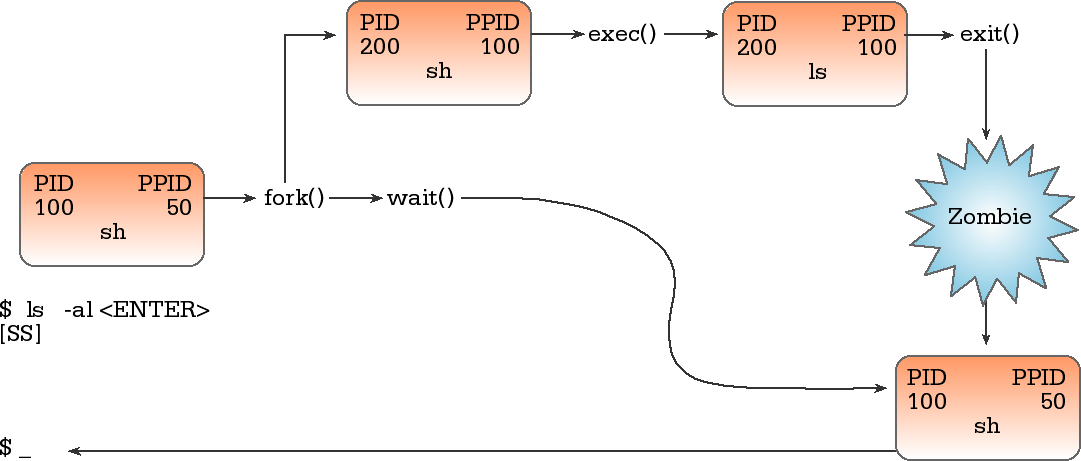
\includegraphics[width=\linewidth]{process_start}
\end{frame}


\begin{frame}[t]
	\frametitle{Interpretori skripti}
	\begin{itemize}
		\item U skriptama se interpretor odabire \emph{shebang} sekvencom znakova \shell{\#!} u prvoj liniji koda
		\begin{itemize}
			\item[] Sintaksa
			\item[] {\ttfamily \#! path [argumenti]}
		\end{itemize}
		\item Shebang sekvenca se može koristiti za odabir interpretora bilo kojeg skriptnog programskog jezika
		\item U shell jezicima se obično navodi kako bi se skripta uvijek pokretala u ispravnoj ljusci
		\item[]
		\item Primjer: U skripti pisanoj za bash (ali ne i za, primjerice, sh) pišemo
		\item[] \ttfamily \#! /bin/bash
	\end{itemize}
\end{frame}

\subsection{Procesi u ljusci}
\begin{frame}[t]
	\frametitle{Posao}
	\begin{itemize}
	  \item Pokretanjem procesa ljuska stvara \emph{posao} (job)
	  \item Posao procesu pridjeljuje atribute kao što su
	  \begin{itemize}
	  	\item Terminal kojem proces (posao) pripada
	  	\item Ulazne i izlazne uređaje (stdin, stdout, stderr)
	  	\item \ldots
	  \end{itemize}
	  \item Posao može objediniti više procesa koji su međusobno ovisni
	  \begin{itemize}
	  	\item[] Primjer: Procesi vezani pipeom objedinjeni su u jedan posao
	  	\item[] \shell{cat /etc/passwd | grep korisnik}
	  \end{itemize}
	  \item Posao ima vlastiti identifikator - \emph{Job ID} (JID)
	  \begin{itemize}
	  	\item Dodjeljuje ga ljuska
	  	\item U svakoj pokrenutoj ljusci brojanje JID-ova počinje od 1 (u dvije ljuske može postojati više istih JID-ova)
	  \end{itemize}
	\item Terminiranjem ljuske terminiraju se svi poslovi u njoj
	\end{itemize}
\end{frame}

\begin{frame}[t]
	\frametitle{Kontrola poslova}
	\begin{itemize}
		\item Posao pokrenut u ljusci može biti u dva načina rada:
		\begin{itemize}
			\item \emph{Foreground} - prednji plan (fokus) u ljuski
			\item \emph{Background} - rad u pozadini
		\end{itemize}
	    \item Kod pokretanja procesa iz terminala ljuska postavlja posao u foreground
	    \item Za pokretanje procesa u pozadini koristi se operator \shell{\&}
	    \item[] Sintaksa: \shell{<naredba> \&}
	    \begin{itemize}
		    \item Ljuska ispisuje JID i PID procesa
	    \end{itemize}
	    \item[]
	    \item[] Primjer: \shell{vim \&}
	    \item[] \hspace{35pt} \shell{[1] 4132}
	\end{itemize}
\end{frame}

\begin{frame}[t]
	\frametitle{Kontrola poslova}
	\begin{itemize}
		\item Proces koji je trenutno u \emph{foreground}-u može se \emph{suspendirati} (signal \shell{SIGTSTP}) kombinacijom tipki \emph{CTRL + Z}
		\item Ljuska ispisuje JID suspendiranog procesa
		\item Proces se može nastaviti naredbama:
		\begin{itemize}
			\item \shell{fg} - u foregroundu
			\item \shell{bg} - u backgroundu
		\end{itemize}
		\item Popis poslova koji se izvode u trenutnoj ljusci dobije se naredbom \shell{jobs}
	\end{itemize}
\end{frame}

\begin{frame}[t]
	\frametitle{Procesi u Linuxu}
	\begin{itemize}
		\item Koncept poslova u ljusci na kernelskoj je razini izveden \emph{grupama procesa}
		\begin{itemize}
			\item Grupe procesa su koncept podržan od samog operativnog sustava
			\item Grupe procesa omogućuju istovremeno slanje signala svim međusobno ovisnim procesima (unutar iste grupe)
			\item U modernim ljuskama ova dva pojma se praktički poistovjećuju
		\end{itemize}
		\item Grupe procesa imaju identifikator PGID (\emph{Process group ID})
		\begin{itemize}
			\item PGID je jednak PID-u prvog pokrenutog procesa u grupi
		\end{itemize}
		\item[]
		\item Osiromašeni (\emph{orphaned}) proces
		\begin{itemize}
			\item Proces koji je ostao pokrenut u grupi procesa nakon što je glavni proces terminiran
		\end{itemize}
	\end{itemize}
\end{frame}


\begin{frame}[t]
	\frametitle{Procesi u Linuxu}
    \begin{itemize}
	    \item Više grupa procesa dio su jedne \emph{sjednice} (engl. \emph{session})
    	\begin{itemize}
    		\item Jedna sjednica obuhvaća sve procese vezane za isti terminal
    		\item Prijavom korisnika na sustav započinje se \emph{login session}
    	\end{itemize}
    \end{itemize}
    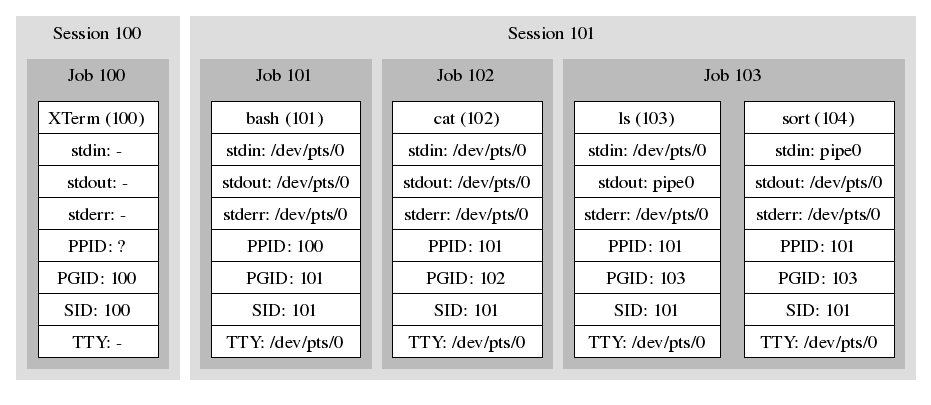
\includegraphics[scale=0.35]{process.png}
\end{frame}


\begin{frame}[t]
	\frametitle{Literatura}
	\begin{itemize}
	  \item \url{http://www.linux.com/archive/feature/125977}
	  \item \url{http://www.linux-tutorial.info/modules.php?name=MContent&pageid=84}
	  \item \url{http://www.linuxhq.com/guides/SAG/x1826.html}
	  \item \url{http://www.win.tue.nl/~aeb/linux/lk/lk-10.html}
	  \item \url{http://www.linusakesson.net/programming/tty/index.php}\\
	  \item \url{http://acms.ucsd.edu/info/jobctrl.html}
	  \item[]
	\end{itemize}
	\shell{man} stranice: \shell{ps}, \shell{7 signal}, \shell{fork} (sva poglavlja), \shell{wait} (sva poglavlja), \shell{jobs}
\end{frame}

\end{document}